%----------------------------------------------------------------------------------------
%	PACKAGES AND OTHER DOCUMENT CONFIGURATIONS
%----------------------------------------------------------------------------------------
\documentclass[13pt]{scrartcl} % Font size
% \documentclass[12pt]{article} % Font size
%----------------------------------------------------------------------------------------
%	PACKAGES AND OTHER DOCUMENT CONFIGURATIONS
%----------------------------------------------------------------------------------------

\usepackage{amsmath, amsfonts, amsthm} % Math packages

% Packages for Title Page
% \usepackage{newlfont}
% \usepackage{gensymb}

% \usepackage{listings} % Code listings, with syntax highlighting

\usepackage[utf8]{inputenc}
% \usepackage[english,vietnam]{babel}
% \usepackage[utf7]{vietnam}

%----------------------------------------------------------------------------------------
%	IMAGES CONFIGURATION
%----------------------------------------------------------------------------------------
\usepackage{graphicx} % Required for inserting images
\graphicspath{{Figures/}{./}} % Specifies where to look for included images (trailing slash required)
\usepackage{xstring}

\usepackage{subcaption}
\DeclareCaptionFormat{custom}
{
    \normalsize\textit{#1}\textit{#2}\textit{\normalsize #3}
}
\captionsetup{format=custom}


%----------------------------------------------------------------------------------------
%	LIST CONFIGURATION
%----------------------------------------------------------------------------------------
% \usepackage{enumitem} % Required for list customisation
% \setlist{noitemsep} % No spacing between list items


%----------------------------------------------------------------------------------------
%	PARAGRAPH FORMATTING 
%----------------------------------------------------------------------------------------
% \setlength\parindent{0pt} % Removes all indentation from paragraphs
% \setlength{\parindent}{2em}
\usepackage{indentfirst}
% \usepackage[skip=10pt plus1pt, indent=25pt]{parskip}

%----------------------------------------------------------------------------------------
%	DOCUMENT MARGINS
%----------------------------------------------------------------------------------------
% \usepackage{geometry} % Required for adjusting page dimensions and margins

% \geometry{
% 	paper=a4paper, % Paper size, change to letterpaper for US letter size
% 	top=2cm, % Top margin
% 	bottom=2.5cm, % Bottom margin
% 	left=3cm, % Left margin
% 	right=3cm, % Right margin
% 	headheight=0.75cm, % Header height
% 	footskip=1.5cm, % Space from the bottom margin to the baseline of the footer
% 	headsep=0.75cm, % Space from the top margin to the baseline of the header
% 	%showframe, % Uncomment to show how the type block is set on the page
% }

%----------------------------------------------------------------------------------------
%	FONTS
%----------------------------------------------------------------------------------------
% \usepackage[utf8]{inputenc} % Required for inputting international characters
% \usepackage[T1]{fontenc} % Use 8-bit encoding
% \usepackage{fourier} % Use the Adobe Utopia font for the document
% \usepackage{sectsty}
\usepackage[usenames,dvipsnames]{color}
% \sectionfont{\fontsize{12}{22}\selectfont}

%----------------------------------------------------------------------------------------
%	SECTION 
%----------------------------------------------------------------------------------------
% \setcounter{section}{14}
% \usepackage{sectsty} % Allows customising section commands

% \sectionfont{\vspace{6pt}\centering\normalfont\scshape} % \section{} styling
% \subsectionfont{\normalfont\bfseries} % \subsection{} styling
% \subsubsectionfont{\normalfont\itshape} % \subsubsection{} styling
% \paragraphfont{\normalfont\scshape} % \paragraph{} styling

%----------------------------------------------------------------------------------------
%	HEADERS AND FOOTERS
%----------------------------------------------------------------------------------------
% \usepackage{scrlayer-scrpage} % Required for customising headers and footers

% \ohead*{} % Right header
% \ihead*{} % Left header
% \chead*{} % Centre header

% \ofoot*{} % Right footer
% \ifoot*{} % Left footer
% \cfoot*{} % Centre footer
 % Include the file specifying the document structure and custom commands
\usepackage[utf8]{vietnam}

\title{Chương 15: Các hệ thống trực quan hóa}
%!TEX encoding = UTF-8 Unicode
\textwidth=450pt\oddsidemargin=5pt
\begin{document}

%----------------------------------------------------------------------------------------
%	TITLE PAGE
%----------------------------------------------------------------------------------------
\begin{titlepage}
    \begin{center}
        {{\Large{\textsc{TRƯỜNG ĐẠI HỌC KHOA HỌC TỰ NHIÊN \\ ĐẠI HỌC QUỐC GIA HÀ NỘI}}}} \rule[0.1cm]{15.8cm}{0.1mm}
        \rule[0.5cm]{15.8cm}{0.6mm}
        {\large{\bf KHOA TOÁN - CƠ - TIN HỌC }}
    \end{center}

    % \vspace{5mm}

    \begin{figure}[!ht] % [!ht] forces the figure to be output where it is defined in the code (it suppresses floating)
        \centering
        
\includegraphics[width=0.25\columnwidth]{hus.jpeg}
    \end{figure}

    % \vspace{5mm}

    \begin{center}
        {\LARGE{\bf CHƯƠNG 15: VISUALIZATION SYSTEMS \\ CÁC HỆ THỐNG TRỰC QUAN HÓA}}
    \end{center}

    \vspace{55mm}

    \hspace{0cm}\begin{minipage}[t]{0.7\textwidth}
        \normalsize{GIẢNG VIÊN:} \\
        \-\hspace{1cm}\large\textbf{TS. Nguyễn Thị Bích Thủy}
    \end{minipage}
    \par

    \vspace{5mm}

    \hspace{0cm}\begin{minipage}[t]{0.7\textwidth}
        \normalsize
        HỌC VIÊN: \\
        \-\hspace{1cm}\large\textbf{Vũ Minh Hưng} \\
        \-\hspace{1cm}\large\textbf{Vũ Trang Linh}
    \end{minipage}
    \par

    \vfill
    \begin{center}
        {\large{\bf Tháng 12 năm 2022 }}
    \end{center}
\end{titlepage}


%----------------------------------------------------------------------------------------
%	TABLE OF CONTENTS
%----------------------------------------------------------------------------------------

% \renewcommand*\contentsname{Summary}
\date{ }
% \maketitle
\tableofcontents

\pagebreak
% \newpage
%----------------------------------------------------------------------------------------
%	INTRODUCTION
%----------------------------------------------------------------------------------------

\section{Lời giới thiệu}
Trong chương này chúng tôi giới thiệu qua một số hệ thống và công cụ trực quan hóa thông tin và dữ liệu. Chúng tôi tập trung ưu tiên các phần mềm miễn phí, cho phép học viên quan tâm tìm hiểu sâu hơn về lĩnh vực trực quan hóa có thể thử nghiệm các công cụ này. Đây chỉ là một số trong rất nhiều các công cụ rất tốt để trực quan hóa dữ liệu mà không được để cập tới trong chương này, bạn độc có thể tự tìm kiếm và tải chúng về dùng thử. Chúng tôi cũng đề cập tới một số công cụ có trả phí mà có các chức năng tương đương với các hệ thống chúng tôi đề cập tới. Lưu ý rằng các đường link của các công cụ là chính xác tại thời điểm xuất bản cuốn sách này, nhưng có thể thay đổi sau này, và một số công cụ có thể không còn được phát hành miễn phí nữa.

%----------------------------------------------------------------------------------------
%	SECTION 1
%----------------------------------------------------------------------------------------

\section{Các hệ thống dựa trên loại dữ liệu}

\subsection{Dữ liệu khoa học}

OpenDX, ban đầu được giới thiệu là một Công cụ khai phá dữ liệu trực quan hóa của IBM, là một môi trường trực quan hóa ban đầu được sử dụng cho phân tích dữ liệu kỹ thuật và khoa học. Cái tách biệt công cụ này với các nền tảng trực quan hóa khá là tiến trình quy hoạch trực quan được sử dụng để tùy biến trực quan hóa. Chức năng Network Editor cho phép người dùng kéo thả các thành phần vào một giao diện và tạo các đường liên kết giữa các thành phần này để biểu diễn sự tương tác dữ liệu tương ứng. Các thành phần thường được xếp vào một vài lớp đối tượng, bao gồm:
\begin{itemize}
    \item Nhập và xuất – các mô đun sử dụng để tải và lưu dữ liệu trong các định dạng khác nhau;
    \item Điều hướng xử lý – các mô đun để tạo các vòng lặp và thực thi theo điều kiện;
    \item Hiện thực hóa – các mô đun để ánh xạ dự liệu vào các thực thể có thể hiển thị, ví dụ như các đẳng diện, lưới, hoặc các đường hướng.
    \item Hiển thị – các mô đun điều khiển các thuộc tính hiển thị, như ánh sáng, góc quay, cắt xén.
    \item Biến đổi – các chức năng áp dụng cho dữ liệu, ví dụ như lọc, các hàm toán học, sắp xếp;
    \item Tương tác – các mô dun như là trình chọn tệp, menu, dial/slider, và các nút bấm.
\end{itemize}

\begin{figure}[!ht] % [!ht] forces the figure to be output where it is defined in the code (it suppresses floating)
    \centering
    
\includegraphics[width=0.7\columnwidth]{1.png}
    \caption{Ví dụ về một mạng lưới trong OpenDX. Luồng xử lý bắt đầu từ mô đun Import tới đầu ra Image.}
\end{figure}

\begin{figure}[!ht] % [!ht] forces the figure to be output where it is defined in the code (it suppresses floating)
    \centering
    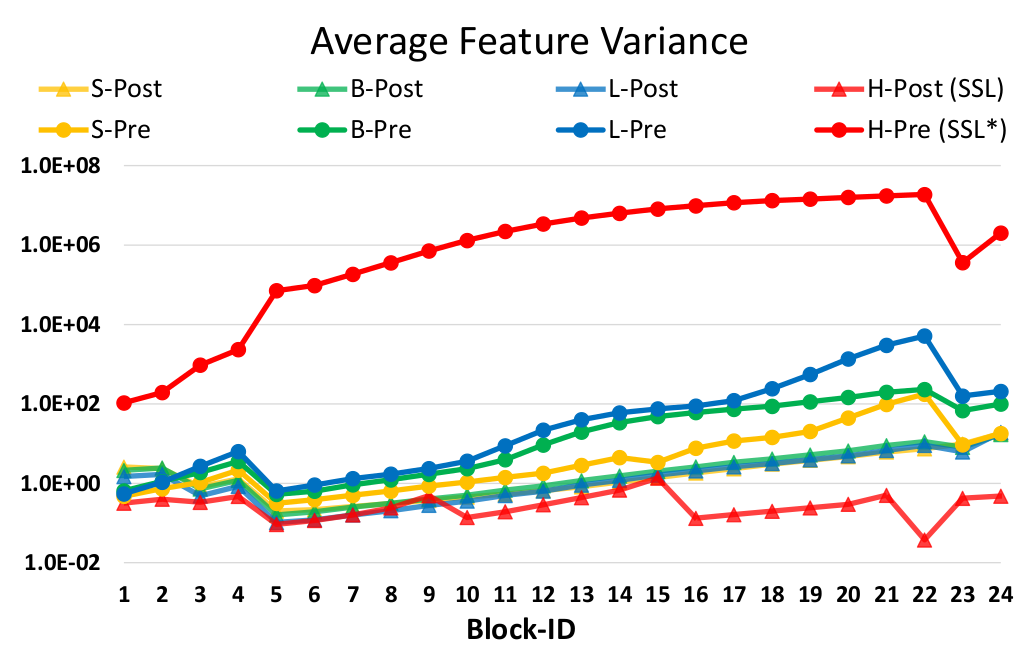
\includegraphics[width=0.8\columnwidth]{2.png}
    \caption{Một ví dụ về giao diện của một mô đun trong OpenDX. Một số tham số cần tự thiết lập, trong khi số khác được thiết lập bằng cách kết nối một tab input hoặc output của một mô đun tới input hoặc output của mô đun khác.}
\end{figure}

\begin{figure}[!ht] % [!ht] forces the figure to be output where it is defined in the code (it suppresses floating)
    \centering
    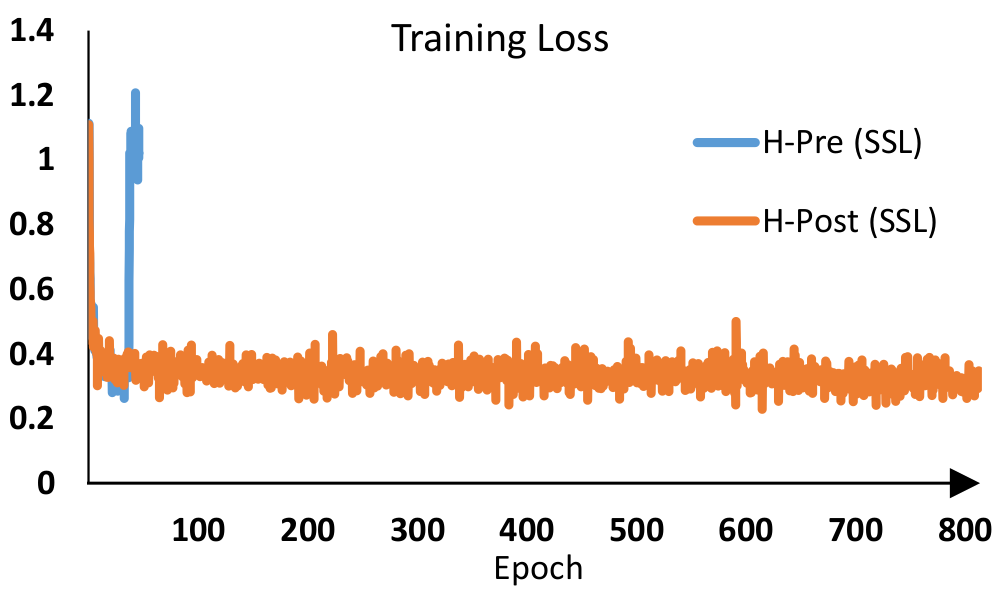
\includegraphics[width=0.7\columnwidth]{3.png}
    \caption{Các ví dụ về trực quan hóa có thể được tạo với OpenDX. Hình đầu kết hợp một mặt cắt qua một trường điện từ, trong khi ở hình thứ 2 kết hợp nhiệt độ, độ ẩm và vùng gió để xem xét các thuộc tính của một đám mây bão.}
\end{figure}

%------------------------------------------------
\newpage
\subsection{Dữ liệu đa biến}

XmdvTool, phát triển bởi Matthew Ward, Elke Rundensteiner và các cộng sự ở Viện Bách Khoa Worcester, là một gói phần mềm trực quan hóa tích hợp năm phương pháp chung cho trực quan hóa dữ liệu đa biến trong một ứng dụng duy nhất. Bộ công cụ này bao gồm ma trận biểu đồ phân tán, biểu đồ phần tán hình sao, các tọa độ song song, xếp chồng theo chiều, và các phương pháp hướng pixel. Các phương pháp trực quan hóa này được liên kết với nhau sử dụng một cơ chế chọn lọc đơn giản gọi là N-dimensional brush, bằng cách định nghĩa một siêu hộp trong không gian dữ liệu. Dữ liệu được lựa chọn trong một view cũng sẽ được chọn trong view khác, và kết quả lựa chọn sẽ được bôi đậm, đánh dấu, xóa đi hoặc phân tích tách rời khỏi toàn bộ dữ liệu.

Ngoài mục tiêu ban đầu, XmdvTool còn được mở rộng để bao gồm thêm các tính năng kiến trúc để hỗ trợ các tập dữ liệu lớn. Ban đầu, Ying Huey Fua giới thiệu hệ tọa độ song song phân cấp cho khai phá dữ liệu có chứa nhiều ghi chép. Dữ liệu được phân cụm theo cấp và kết quả được hiển thị trong một hệ tọa độ song song sử dụng độ trong suốt là biến số. Sau đó công cụ được thêm brush dựa trên cấu trúc, là một giao diện người dùng tích hợp cho duyệt và vẽ bên trong cấu trúc dữ liệu phân cấp. Jing Yang sau đố tổng quát hóa ứng dụng của cấu trúc dữ liệu phân cấp này với các công cụ trực quan hóa khác của XmdvTool và định nghĩa ra framework hiển thị phân cấp tương tác. Thêm vào đó, XmdvTool cung cấp một framework giảm chiều phân cấp trực quan mà có thể nhóm lại và tổ chức không gian các chiều, cung cấp các không gian con có ý nghĩa cho việc phân tích. XmdvTool cũng bao gồm cách tiếp cận phân lớp số lượng theo khoảng cách để xử lý các biến danh nghĩa và các công cụ để sắp xếp lại các chiều để giảm sự lộn xộn trực quan.

\begin{figure}[!ht] % [!ht] forces the figure to be output where it is defined in the code (it suppresses floating)
    \centering
    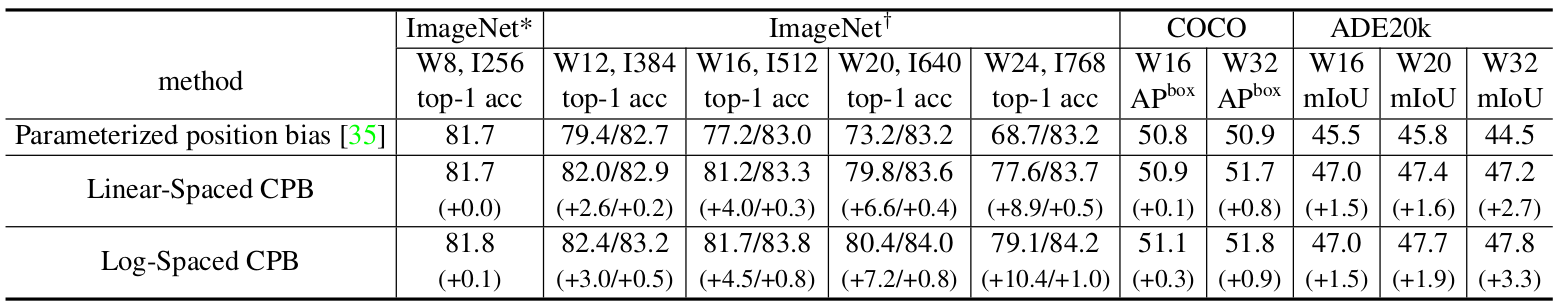
\includegraphics[width=0.8\columnwidth]{4.png}
    \caption{Ví dụ về hệ tọa độ song song phân cấp trong XmdvTool. Mỗi đường mảnh đại diện cho tâm của một nhóm, và dải mờ quanh mỗi đường trung tâm chỉ phạm vi của nhóm trong mỗi chiều. Vùng mờ gần tâm để chỉ dân số của mỗi nhóm. }
\end{figure}


XmdvTool được giới thiệu lần đầu vào năm 1994, và tại thời điểm viết cuốn sách này, nó ở phiên bản 7.0. Ngoài định dạng file của ứng dụng, nó có thể hỗ trợ bảng biểu Excel hoặc cơ sở dữ liệu Oracle. Ứng dụng này được ứng dụng rộng rãi trong các ứng dụng như khoa học không gian và trái đất, sinh tin học, nghiên cứu dân số và phân tích hiệu năng của mạng lưới.

\begin{figure}[!ht] % [!ht] forces the figure to be output where it is defined in the code (it suppresses floating)
    \centering
    \includegraphics[width=0.8\columnwidth]{5.png}
    \caption{Hiển thị các cấu trúc phân cấp trong XmdvTool. Hình đầu là brush dựa trên cấu trúc sử dụng để điều hướng và lựa chọn trong một phân cấp dữ liệu. Hình thứ hai là InterRing, cho phép người dùng phân loại các chiều dữ liệu và lựa chọn tập con hoặc trung bình các chiều cho hiển thị dữ liệu.}
\end{figure}

Một số phần mềm có chức năng tương tự với XmdvTool bao gồm Spotfire, và Tableau (có trả phí), các phần mềm này đều có nhiều chức năng hơn XmdvTool.

%------------------------------------------------

\subsection{Dữ liệu đồ thị}

GraphViz là một thư viện các thuật toán dựa trên đồ thị phát triển ở Viện Nghiên cứu ATT. Kiến trúc và triết lý của GraphViz là khá độc nhất khi so sánh với các công cụ trực quan hóa khác. Nó hỗ trợ một loạt các phương pháp chuyên cho đồ thị, các phương pháp trình bày và các phương pháp hiển thị. Tong khi một số thành phần tương tác đã được tích hợp trong hệ thống, phần mềm này chủ yếu vẫn thiên về dòng lệnh. Người dùng lựa chọn một tệp mô tả đồ thị và truyền vào mô đun trình bay, cùng với định dạng đầu ra mong muốn. Định dạng đầu ra được hỗ trợ rất nhiều và dễ dàng ích hợp các kết quả vào các tài liệu, website và ứng dụng.

Tất cả các chương trình GraphViz yêu cầu tệp truyền vào ở dạng ngôn ngữ DOT, bên dưới là một ví dụ của đồ thị định nghĩa trong ngôn ngữ DOT:

\begin{figure}[!ht] % [!ht] forces the figure to be output where it is defined in the code (it suppresses floating)
    \centering
    \includegraphics[width=0.45\columnwidth]{6.png}
\end{figure}

Mỗi dòng định nghĩa các thuộc tính của một đồ thị gồm các đỉnh, các cạnh. Cả đồ thị vô hướng và có hướng đều được hỗ trợ. Hình 15.6 bên dưới sử dụng bốn kiểu trình bày đồ thị, bao gồm:
\begin{itemize}
    \item Dot – tiếp cận theo lớp, độ thị có các cạnh theo cùng một hướng.
    \item Neato – mô hình dựa trên mở rộng đa chiều
    \item Circos – trình bày theo vòng tròn, thương hiệu quả cho các mạng thông tin.
    \item Fdp – phương pháp hướng lực sử dụng phỏng đoán đa lưới, cho phép biểu diễn được các đồ thị rất lớn.
\end{itemize}

\begin{figure}[!ht] % [!ht] forces the figure to be output where it is defined in the code (it suppresses floating)
    \centering
    \includegraphics[width=0.8\columnwidth]{7.png}
    \caption{Đầu ra của GraphViz, đại diện cho một đồ thị với 4 cách trình bày khác nhau.}
\end{figure}

Công cụ khác cũng sử dụng để biểu diễn đồ thị là Tom Sawyer Sofware (có mất phí).


%----------------------------------------------------------------------------------------
%	SECTION 2
%----------------------------------------------------------------------------------------
\section{Các hệ thống dựa trên loại phân tích}
\subsection{Thống kê}
GGobi là một công cụ tương tác cho phân tích và trực quan hóa dữ liệu đa biến phát triển bởi Deborah Swayne, Dianne Cook và Andreas Buja vào đầu những năm 1990 tại Bellcore, Inc. Nó hỗ trợ một số phương pháp trực quan hóa, bao gồm biểu đồ phân tán, ma trận biểu đồ phân tán, biểu đồ cột, đồ thị và các tọa độ song song (xem hình 15.7).

\begin{figure}[!ht] % [!ht] forces the figure to be output where it is defined in the code (it suppresses floating)
    \centering
    \includegraphics[width=0.8\columnwidth]{8.png}
    \caption{Ví dụ về các tọa độ song song trong ứng dụng GGobi.}
\end{figure}

Với mỗi phương pháp trực quan hóa, bản điều khiển tương ứng sẽ được hiển thị bằng cách ấn vào phương pháp đó. Màu sắc được sử dụng để liên kết dữ liệu giữa nhiều phần hiển thị, và người dùng sẽ có nhiều tùy chọ để điều chỉnh màu sắc tương ứng với mỗi thực thể đồ họa. Người dùng bắt đầu bằng việc lựa chọn một chiều dữ liệu để điều chỉnh màu sắc, một biểu đồ histogram có thể được sử dụng để điều chỉnh khoảng giá trị gán với mỗi màu (hình 15.8). Bôi màu được liện kết có thể được sử dụng để bôi đậm một điểm dữ liệu được lựa chọn ở mỗi màn hình.

\begin{figure}[!ht] % [!ht] forces the figure to be output where it is defined in the code (it suppresses floating)
    \centering
    \includegraphics[width=0.8\columnwidth]{9.png}
    \caption{Bôi màu được chỉnh tự động trong GGobi. Người dùng có thể gán bất cứ chiều dữ liệu nào để điều chỉnh màu sắc và có thể điều chỉnh khoảng màu được sử dụng.}
\end{figure}

Một trong những công cụ mạnh mẽ nhất trong ứng dụng GGobi là khả năng tạo và xem “grand tours” của dữ liệu, sử dụng một đường qua không gian chiếu để trình chiếu dữ liệu ở tất cả các view, hoặc từ các tập con ràng buộc với người dùng ở mỗi view. Người dùng có thể thay đổi tốc độ chuyển động và dừng lại để kiểm tra các đặc trưng mong muốn, cũng như xem các tham số mà tạo ra các view.

Nhiều công cụ khác đã được thêm vào GGobi trong thời gian dài, bao gồm liên kết với các gói thư viện thống kê bằng ngôn ngữ R, hỗ trợ cho vài phương pháp vẽ đồ thị (xem hình 15.9), các phương pháp để xử lý dữ liệu bị thiếu, các phương pháp giảm chiều dữ liệu như PCA và MDS.

\begin{figure}[!ht] % [!ht] forces the figure to be output where it is defined in the code (it suppresses floating)
    \centering
    \includegraphics[width=0.7\columnwidth]{10.png}
    \caption{Ví dụ về vẽ đồ thị trong GGobi. Trình bày theo hình tỏa tròn là một trong vài cách trình bày được hỗ trợ.}
\end{figure}

Phần mềm có thể chạy trên Windows, Mac và Linux. Code, tệp thực thi, tài liệu và các hỗ trợ khác có thể được tìm thấy trên website của GGobi.

Các phần mềm khác dùng cho phân tích và đồ thị thống kê bao gồm SPSS (trả phí), và SAS (trả phí), và những phần mềm này có nhiều chức năng hơn là chỉ trực quan hóa thống kê.


%------------------------------------------------

\subsection{Không gian - Thời gian}
Macrofocus đã phát triển một số công cụ tương tác mạnh mẽ cho khai phá dữ liệu và thông tin một cách trực quan. Một trong số đó là InfoScope, liên kết các view địa lý với một vài các biểu diễn bằng hình ảnh hoặc chữ. Một ví dụ của màn hình chính của InfoScope được biểu diễn ở 0. Trong ví dụ này, thông tin từ Liên hợp quốc về phát triển con người có thể được khai phá bằng nhiều cách khác nhau.

\begin{figure}[!ht] % [!ht] forces the figure to be output where it is defined in the code (it suppresses floating)
    \centering
    \includegraphics[width=0.8\columnwidth]{11.png}
    \caption{Một ví dụ về màn hình của InfoScope.}
\end{figure}

View địa lý (1) chỉ ra view toàn cầu hoặc view địa phương của các thành phần địa lý trong tập dữ liêu. Một ống kính mắt cá được sử dụng để thu phóng giữ ngữ cảnh bằng cách giữ chuột.

\begin{figure}[!ht] % [!ht] forces the figure to be output where it is defined in the code (it suppresses floating)
    \centering
    \includegraphics[width=0.8\columnwidth]{12.png}
    \caption{View địa lý trong InfoScope: người dùng có thể lựa chọn các nút cho trước hoặc ấn vào vị trí trên bản đồ.}
\end{figure}

View chủ đề (2) trình chiếu các điểm dữ liệu được trình bày dựa trên sự tương tự sử dụng một thuật toán MDS tối ưu.

\begin{figure}[!ht] % [!ht] forces the figure to be output where it is defined in the code (it suppresses floating)
    \centering
    \includegraphics[width=0.5\columnwidth]{13.png}
    \caption{View theo chủ đề trong InfoScope: người dùng có thể lựa chọn từ một số các cách trình bày khác nhau mà biểu diễn mối liên hệ giữa các dữ liệu.}
\end{figure}

View dữ liệu (3) có thể thể hiện dữ liệu hoặc dưới dạng tọa độ song song hoặc bảng biểu.

\begin{figure}[!ht] % [!ht] forces the figure to be output where it is defined in the code (it suppresses floating)
    \centering
    \includegraphics[width=0.8\columnwidth]{14.png}
    \caption{View đồ họa trong InfoScope, với các tọa độ song song để vẽ dữ liệu. Các dữ liệu thấp hơn trên một trong các chiều đã bị lọc đi, kết quả là màu tối cho những dữ liệu này trong các view.}
\end{figure}


Sức mạnh của InfoScope nằm ở liên kết chặt chẽ của nó với các view khác nhau. Bôi màu trong bất cứ view nào sẽ bôi đâm dữ liệu tương ứng trong tất cả các view còn lại. Lên tới 4 loại bút tô có thể được sử dụng để tách biệt từng ghi chép cho hiển thị song song. Dữ liệu có thể dược lọc bằng cách kéo các trình điều khiển ở trên hoặc dưới cùng của mỗi trục tọa độ song song để cho phép người dùng làm mờ đi các giá trị cao hoặc thấp. Màu sắc có thể được liên kết với bất cứ biến dữ liệu nào, vì vậy người dùng có thể dễ dàng chuyển đổi giữa các bản đồ theo chủ đề khác nhau. Di chuột qua các điểm dữ liệu sẽ hiện lên nhãn hoặc giá trị một cách trực quan.

Các hiệu ứng chuyển động cũng được sử dụng hiệu quả trong InfoScope. Các chức năng thu phóng trong mỗi màn hình được thực thi một cách liền mạch, cho phép người dùng dễ dàng theo sát ngữ cảnh. Các chiều dữ liệu trong các tọa độ song song có thể được co lại hoặc dãn ra giúp dễ dàng phân tích. Trong view chủ đề, chuyển đổi giữa các chủ đề khác nhau tạo ra một hiệu ứng liền mạch về sự chuyển động của các điểm dữ liệu, cho phép người dùng tách biệt các mối quan hệ mà bất biến tương đối giữa các chủ đề với các điểm dữ liệu mà khác biệt đáng kể dựa trên chủ đề.

Phần mềm Macrofocus không hẳn là phần mềm miễn phí; công ty phân phối tệp thực thi miễn phí và cho phép người dùng khám phá một số tập dữ liệu mà Macrofocus cung cấp, nhưng để nhập vào dữ liệu của mình, thì người dùng cần phải trả phí qua trang web của công ty.

Trực quan hóa không- thời gian là một thế mạnh của các hệ thống thống tin theo địa lý. Bên cạnh InfoScope, còn có một số phần mềm khác như là GRASS, ArcGIS, và ERDAS IMAGINE.



%----------------------------------------------------------------------------------------
%	SECTION 3
%----------------------------------------------------------------------------------------
\section{Phân tích và trực quan hóa dữ liệu dạng text}
Jigsaw là một công cụ trực quan hóa dữ liệu dạng text được phát triển bởi John Stasko và các cộng cự ở Viện công nghệ Georgia. Hệ thống này khai phá các thực thể (người, nơi chốn, ngày, tiền tệ) và các mối quan hệ giữa chúng. Jigsaw sử dụng một vài view khác nhau để biểu diễn dữ liệu tới người dùng bao gồm lịch, danh sách, đồ thị, biểu đò phân tán, text và các view theo thời gian, như được trình bày ở 4. Mỗi view được biểu diễn như là một cửa sổ riêng biệt mà cập nhật tự động với các kết quả của query khác nhau.


\begin{figure}[!ht] % [!ht] forces the figure to be output where it is defined in the code (it suppresses floating)
    \centering
    \includegraphics[width=0.8\columnwidth]{15.png}
    \caption{Ví dụ về các view khác nhau trong Jigsaw. Tương ứng là view dạng danh sách, dạng biểu đồ phân tán, đồ thị và theo thời gian.}
\end{figure}

\begin{figure}[!ht] % [!ht] forces the figure to be output where it is defined in the code (it suppresses floating)
    \centering
    \includegraphics[width=0.8\columnwidth]{16.png}
    \caption{Ví dụ về cấu hình màn hình sử dụng trong Jigsaw. }
\end{figure}

Tất cả các view được liên kết mặc định với nhau, vậy nên thao tác trên một tài liệu hoặc thực thể ở mỗi view sẽ khiến cho các màn hình khác cập nhật tương ứng. Việc cập nhật có thể ddowwjc bật hoặc tắt ở bất cứ màn hình nào để lưu giữ trạng thái của nó. Nó thường hữu ích khi thực sự chứng kiến các view khi chúng cập nhật, để dễ dàng thấy được chúng thay đổi như thế nào. Người dùng có thể thấy việc cần thiết khi sử dụng Jigsaw với 4 hoặc nhiều màn hình hơn, như ở 5., để thu được hết lợi ích của hệ thống.

Công cụ này đặc biệt hữu ích trong khai phá dữ liệu liên quan tới một tập lớn các dữ liệu và thông tin. Các ứng dụng của nó bao gồm tình báo quân sự, thi hành luật pháp, báo chí, hoặc các lĩnh vực tương đương. Cũng quan trọng khi chỉ ra rằng trong khi công cụ này có thể giúp phân tích trên một số lượng lớn tài liệu, các thực thể và mối quạn hệ giữa chúng, nó không thể thay thế được việc thực sự đọc các tài liệu này. Ví dụ, nó có thể giúp một nhà phân tích xác định tài liệu nào là quan trọng và cần được đọc, giúp tiết kiệm thời gian thay vì đọc toàn bộ tài liệu, điều mà khó khả thi.
\end{document}